\documentclass[12pt, a4paper, oneside]{ctexart}
\usepackage{amsmath, amsthm, amssymb, bm, color, framed, graphicx, hyperref, mathrsfs, mathtools, enumerate, tikz}
\usepackage{float}
\usepackage{subcaption} 



\usetikzlibrary{patterns}

\title{\textbf{Homework 7}}
\author{萃英学院\qquad 2022级\qquad 王一鑫}
\date{\today}
\linespread{1.5}
\newcounter{problemname}
\newenvironment{problem}{\begin{framed}\stepcounter{problemname}\par\noindent\textsc{Problem \arabic{problemname}. }}{\end{framed}\par}
\newenvironment{solution}{%
	\par\noindent\textsc{Solution. }\ignorespaces
}{%
	\hfill$\qed$\par
}
\newenvironment{note}{\par\noindent\textsc{Note of Problem \arabic{problemname}. }}{\\\par}

\begin{document}
	
	\maketitle
	
	\begin{problem}
		
    A topological space is \textbf{totally disconnected} if all of its components are singletons.

    \begin{enumerate}[(1)]
        \item The subset $\mathbb{Q}$ of all rational numbers is a subspace of one-dimensional Euclidean space $\mathbb{R}^1$. Prove that $\mathbb{Q}$ is totally disconnected.
        \item Is $\mathbb{Q}$ discrete?
        \item Prove that the Cantor set is totally disconnected.
    \end{enumerate}
        
	\end{problem}
    
	\begin{solution}
        
	    \begin{enumerate}[(1)]
            \item if $C \subseteq \mathbb{Q}$ and $q_1 < q_2$ exist in $C$, we can find an irrational 
            $s$ in between and then $\{ (-\infty, s) \cap \mathbb{Q}, (s, \infty) \cap \mathbb{Q} \}$ 
            disconnects $\mathbb{Q}$ and $C$. So any subset of $\mathbb{Q}$ with two or more points is disconnected.

            \item In the subspace topology, a singleton $\{q\}$ in $\mathbb{Q}$ would need to be the intersection of 
            an open set in $\mathbb{R}$ with $\mathbb{Q}$.

            Any open set in $\mathbb{R}$ containing $q$ must contain an interval around $q$, 
            which includes infinitely many rational numbers. Hence, singletons in $\mathbb{Q}$ are not open.
            Since $\mathbb{Q}$ has no isolated points, it is not discrete.
            
            \item Consider two distinct points $x$ and $y$ in the Cantor set $C$. 
            Their ternary expansions differ at some position $n$.

            At the $n$-th stage of the Cantor set construction, the interval containing $x$ and $y$ is split, 
            and the middle third is removed, placing $x$ and $y$ in different intervals.
            
            These intervals are clopen in $C$, allowing $x$ and $y$ to be separated by clopen sets. 
            Thus, the connected component of $x$ cannot contain $y$, showing all components are singletons. 
            Hence, $C$ is totally disconnected.
            
        \end{enumerate}
		
	\end{solution}
		

		
	
	\begin{problem}
		(Exercise 4.18)

        Let \( M_1 \) and \( M_2 \) be \( n \)-manifolds. For \( i = 1, 2 \), 
        let \( B_i \subseteq M_i \) be regular coordinate balls, and 
        let \( M_i' = M_i \setminus B_i \). Choose a homeomorphism 
        \( f : \partial M_2' \to \partial M_1' \) 
        (such a homeomorphism exists by Problem 4-17). 
        Let \( M_1 \# M_2 \) (called a \textbf{connected sum of \( M_1 \) 
        and \( M_2 \)}) be the adjunction space \( M_1' \cup_f M_2' \) 
        (Fig. \ref{fig:CS}).

        \begin{enumerate}
            \item[(a)] Show that \( M_1 \# M_2 \) is an \( n \)-manifold (without boundary).
            \item[(b)] Show that if \( M_1 \) and \( M_2 \) are connected and \( n > 1 \), then \( M_1 \# M_2 \) is connected.
            \item[(c)] Show that if \( M_1 \) and \( M_2 \) are compact, then \( M_1 \# M_2 \) is compact.
        \end{enumerate}
        
        \begin{figure}[H]
			\small
			\centering
			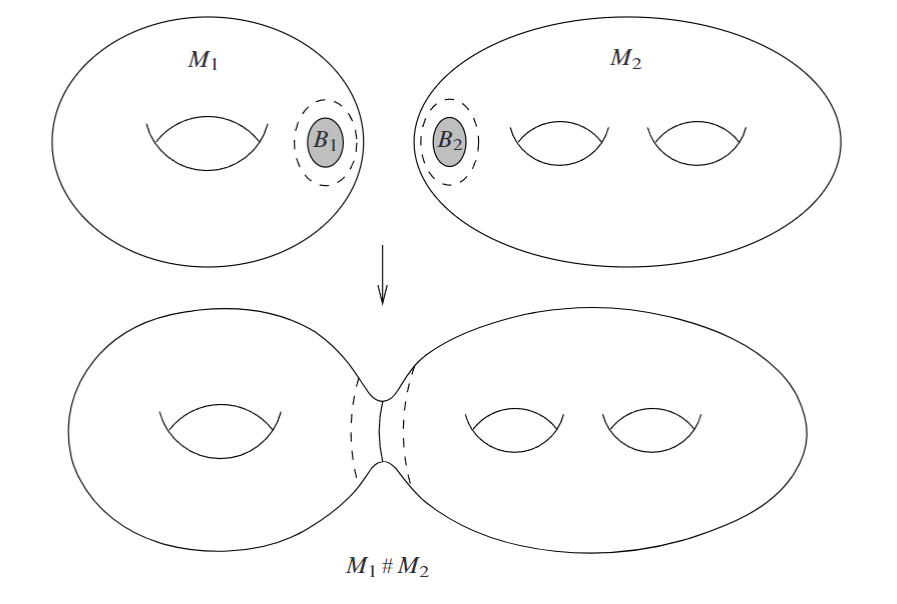
\includegraphics[width=0.8\columnwidth]{figure/fig1.png}
			\caption{Connected Sum}
			\label{fig:CS}
		\end{figure}

	\end{problem}
	
	\begin{solution}
		
        \begin{enumerate}[(a)]
            \item For points in the interior of $M_1'$ or $M_2'$, neighborhoods remain homeomorphic to $\mathbb{R}^n$.

                For points on the glued boundary, consider collar neighborhoods around $\partial M_1'$ and $\partial M_2'$. These collars, homeomorphic to $S^{n-1} \times [0,1]$ and $S^{n-1} \times (-1,0]$, merge to form $S^{n-1} \times (-1,1)$. Using the radial extension of the homeomorphism $f$, this merged neighborhood is homeomorphic to $\mathbb{R}^n$. Thus, every point in $M_1 \# M_2$ has a neighborhood homeomorphic to $\mathbb{R}^n$, making it an $n$-manifold without boundary.
            
            \item A theorem from the book furnishes topological embeddings 
                \[
                e_i : M_i' \to M_1 \# M_2 \quad \text{such that:}
                \]
                \[
                e_1(M_1') \cup e_2(M_2') = M_1 \# M_2
                \]
                \[
                e_1(M_1') \cap e_2(M_2') = e_1(\partial M_1') = e_2(\partial M_2')
                \]
                Since the $M_i'$ have nonempty boundary, $e_1(M_1') \cap e_2(M_2') \neq \emptyset$. Now, $e_i(M_i')$ being a topological embedding, it is connected if and only if $M_i'$ is connected, which is true if $M_i$ is connected.

                So assuming that $M_1$ and $M_2$ are connected, this shows that $M_1 \# M_2$ is the union of nonempty connected sets with nonempty intersection, which implies that it is connected.
            \item 
            $M_1'$ and $M_2'$ are compact as they are closed subsets of compact manifolds.

            The adjunction space $M_1' \cup_f M_2'$ is a quotient of the compact space $M_1' \sqcup M_2'$, hence compact.

        \end{enumerate}
        
		
	\end{solution}
	
	\begin{problem}
        (Exercise 6.1)

        Show that a connected sum of one or more projective planes contains 
        a subspace that is homeomorphic to the M\"obius band.
       
	\end{problem}
	
	\begin{solution}
       By Fig \ref{fig:3} from Wikipedia we know that the right diagram is the subset of the left diagram.
        \begin{figure}[H]
			\small
			\centering
			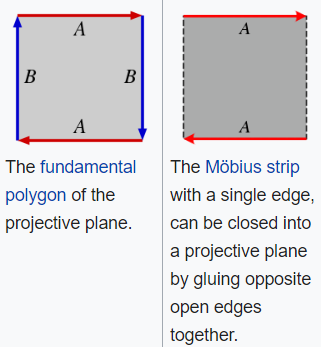
\includegraphics[width=0.35\columnwidth]{figure/fig4.png}
			\caption{Projective planes vs M\"obius band}
			\label{fig:3}
		\end{figure}
        
	\end{solution}
	
	
	
	\begin{problem}
        (Exercise 6.2) 
        
        Note that both a disk and a M\"obius band are manifolds with boundary, 
        and both boundaries are homeomorphic to \(\mathbb{S}^1\). Show that 
        it is possible to obtain a space homeomorphic to a projective plane 
        by attaching a disk to a M\"obius band along their boundaries.

		
	\end{problem}
	
	\begin{solution}
        
        To see that $P^2$ minus a disk is a Mobius band, see Fig \ref{fig:4}. 
        In the upper left is $P^2$, drawn as a fundamental polygon with sides identified. 
        In the upper right, we've removed a disk. The boundary of the now-missing disk is drawn 
        at the lower left as a dashed line. In the lower right we obtain the required M\"obius band. 
        \begin{figure}[H]
			\small
			\centering
			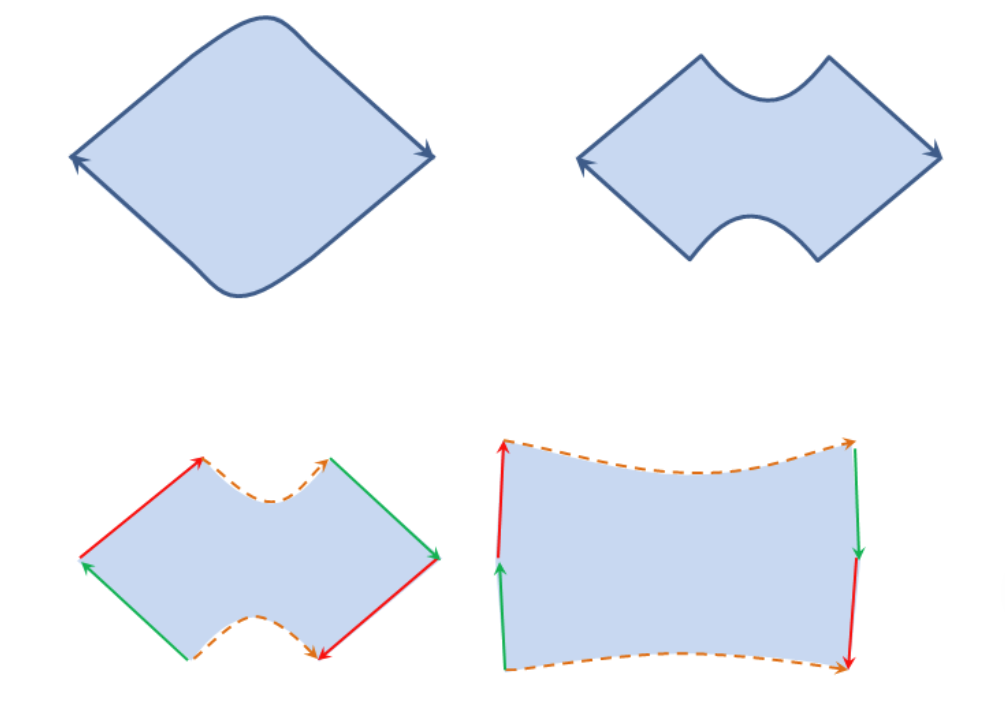
\includegraphics[width=0.8\columnwidth]{figure/fig2.png}
			\caption{Construction}
			\label{fig:4}
		\end{figure}

	\end{solution}


	\begin{problem}
		(Exercise 6.3)

        Show that the Klein bottle is homeomorphic to a quotient obtained 
        by attaching two M\"obius bands together along their boundaries.
        
    \end{problem}

    \begin{solution}
        See Fig \ref{fig:5}.
        \begin{figure}[H]
			\small
			\centering
			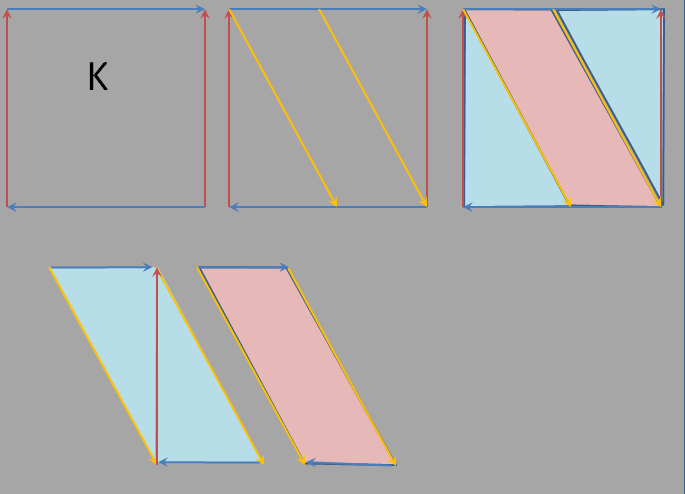
\includegraphics[width=0.8\columnwidth]{figure/fig3.png}
			\caption{Construction}
			\label{fig:5}
		\end{figure}
    \end{solution}
\end{document}


